\documentclass[]{article}
\usepackage[T1]{fontenc}
\usepackage[utf8]{inputenc}
\usepackage{lmodern}
\usepackage[a4paper]{geometry}
\usepackage{polski}
\usepackage{tocloft}
\usepackage{fancyhdr}
\usepackage{graphicx}

% opening
\title{Milionerzy - Projekt Politechnika Lubelska}
\author{Mateusz Walo, Igor Kozak, Oskar Wilkos}
\date{}

\begin{document}
	
	% Tytuł dokumentu
	\maketitle
	
	\begin{center}
		
\includegraphics[width=0.35\textwidth]{pl.jpg} 
	\end{center}
	
	% Spis treści
	\tableofcontents
	\newpage
	
	% Nagłówki
	\fancyhf{} % Resetuje domyślny styl nagłówków i stopek
	\fancyhead[L]{\bfseries Milionerzy - Projekt Politechnika Lubelska} % Nagłówek po lewej stronie
	\pagestyle{fancy}
	\renewcommand{\cftsecfont}{\bfseries} % Czcionka sekcji
	\setlength{\cftsecnumwidth}{2.5em} % Odstęp w numerach sekcji
	
	% Sekcja 1
	\section{Ogólny opis aplikacji}
	Aplikacja jest inspirowana popularną grą \emph{„Milionerzy”} i umożliwia użytkownikowi odpowiadanie na pytania quizowe. Gra oferuje dwa koła ratunkowe: „50/50” i „Telefon do przyjaciela”. Rozgrywka kończy się, gdy użytkownik zdobędzie 1000 punktów, co oznacza zwycięstwo. Każda poprawna odpowiedź daje 100 punktów. Po zakończeniu gry, użytkownik może rozpocząć nową rundę. Aby zmienić poziom trudności, należy zamknąć grę i uruchomić ją ponownie.
	
	\newpage
	
	% Sekcja 2
	\section{Struktura kodu}
	
	\subsection{Nagłówki i biblioteki}
	
	Kod rozpoczyna się od dołączenia wymaganych bibliotek oraz plików nagłówkowych. Główne użyte elementy to:
	
	\begin{itemize}
		\item \texttt{\#include "ProjektMain.h"} - Plik nagłówkowy projektu.
		\item \texttt{\#include <wx/msgdlg.h>} - Biblioteka WX Widgets do obsługi okien dialogowych.
		\item \texttt{\#include <nlohmann/json.hpp>} - Biblioteka JSON do obsługi plików będących bazami pytań.
		\item \texttt{\#include <random>} - Obsługa generowania losowych wartości.
		\item \texttt{\#include <algorithm>} - Obsługa metod wykorzystanych do losowania pytań.
	\end{itemize}
	
	Struktura \texttt{Question} przechowuje dane pojedynczego pytania quizowego:
	
	\begin{itemize}
		\item \texttt{std::string tresc} - Treść pytania.
		\item \texttt{std::vector<std::string> odpowiedzi} - Lista możliwych odpowiedzi.
		\item \texttt{std::string poprawna\_odpowiedz} - Poprawna odpowiedź.
	\end{itemize}
	
	\subsection{Zmienne globalne}
	
	Następnie zdefiniowane są zmienne globalne używane w aplikacji:
	
	\begin{itemize}
		\item \texttt{std::vector<Question> questions} - Lista wszystkich pytań.
		\item \texttt{std::vector<bool> askedQuestions} - Informacja o tym, które pytania zostały już zadane.
		\item \texttt{size\_t currentQuestionIndex} - Indeks bieżącego pytania.
		\item \texttt{bool fiftyFiftyUsed, phoneAFriendUsed, fiftyFiftyUsedGlobal, phoneAFriendUsedGlobal} - Flagi użycia kół ratunkowych.
		\item \texttt{int points} - Aktualna liczba punktów użytkownika.
	\end{itemize}
	
	\subsection{Funkcja \texttt{wxbuildinfo}}
	
	Funkcja \texttt{wxbuildinfo} zwraca informacje o kompilacji aplikacji:
	
	\begin{itemize}
		\item Argument \texttt{format} określa, czy zwracane informacje mają być w formacie krótkim, czy długim.
		\item Funkcja wykorzystuje makra preprocesora do dodania informacji o systemie operacyjnym i trybie kompilacji (Unicode/ANSI).
	\end{itemize}
	
	\begin{verbatim}
		wxString wxbuildinfo(wxbuildinfoformat format)
		{
			wxString wxbuild(wxVERSION_STRING);
			
			if (format == long_f)
			{
				#if defined(__WXMSW__)
				wxbuild << _T("-Windows");
				#elif defined(__UNIX__)
				wxbuild << _T("-Linux");
				#endif
				
				#if wxUSE_UNICODE
				wxbuild << _T("-Unicode build");
				#else
				wxbuild << _T("-ANSI build");
				#endif // wxUSE_UNICODE
			}
			
			return wxbuild;
		}
	\end{verbatim}
	
	\subsection{Klasa \texttt{ProjektDialog}}
	
	Klasa \texttt{ProjektDialog} reprezentuje główne okno dialogowe aplikacji:
	
	\subsubsection{Konstruktor i destruktor}
	
	Konstruktor inicjalizuje interfejs użytkownika oraz ładuje pytania na podstawie wybranego poziomu trudności. Destruktor jest pusty i nie zawiera żadnej dodatkowej logiki.
	
	\subsubsection{Metoda \texttt{OnPaint}}
	
	Metoda \texttt{OnPaint} odpowiada za rysowanie tła okna:
	
	\begin{verbatim}
		void ProjektDialog::OnPaint(wxPaintEvent& event)
		{
			wxPaintDC dc(this);
			
			wxBitmap backgroundBitmap(wxT("resources/kosmos.jpg"), wxBITMAP_TYPE_JPEG);
			
			wxImage scaledImage = backgroundBitmap.ConvertToImage();
			scaledImage = scaledImage.Scale(GetSize().GetWidth(), GetSize().GetHeight());
			
			dc.DrawBitmap(wxBitmap(scaledImage), 0, 0, true);
			
			event.Skip();
		}
	\end{verbatim}
	
	\subsubsection{Metoda \texttt{DisplayQuestion}}
	
	Metoda \texttt{DisplayQuestion} wyświetla bieżące pytanie:
	
	\begin{verbatim}
		void ProjektDialog::DisplayQuestion()
		{
			if (questions.empty())
			{
				wxMessageBox(_("Brak pytań! :( "), _("Error"), wxOK | wxICON_ERROR);
				return;
			}
			
			std::random_device rd;
			std::mt19937 gen(rd());
			std::uniform_int_distribution<> dis(0, questions.size() - 1);
			do {
				currentQuestionIndex = dis(gen);
			} while (askedQuestions[currentQuestionIndex]);
			
			askedQuestions[currentQuestionIndex] = true;
			Question& question = questions[currentQuestionIndex];
			
			std::vector<std::string> shuffledAnswers = question.odpowiedzi;
			
			std::shuffle(shuffledAnswers.begin(), shuffledAnswers.end(), gen);
			
			TextCtrl1->SetValue(wxString::FromUTF8(question.tresc));
			Button1->SetLabel(wxString::FromUTF8(shuffledAnswers[0]));
			Button2->SetLabel(wxString::FromUTF8(shuffledAnswers[1]));
			Button3->SetLabel(wxString::FromUTF8(shuffledAnswers[2]));
			Button4->SetLabel(wxString::FromUTF8(shuffledAnswers[3]));
			
			fiftyFiftyUsed = false;
			phoneAFriendUsed = false;
		}
	\end{verbatim}
	
	\subsubsection{Metoda \texttt{LoadQuestionsFromFile}}
	
	Metoda \texttt{LoadQuestionsFromFile} ładuje pytania z pliku JSON. Jest to kluczowy element aplikacji, który pozwala na dynamiczne wczytywanie pytań na podstawie wybranego poziomu trudności.
	
	\begin{verbatim}
		void ProjektDialog::LoadQuestionsFromFile(const wxString& fileName)
		{
			std::ifstream file(fileName.ToStdString());
			if (file.is_open())
			{
				json jsonData;
				file >> jsonData;
				questions.clear();
				askedQuestions.clear();
				for (const auto& item : jsonData["pytania"])
				{
					Question q;
					q.tresc = item["tresc"];
					q.odpowiedzi = item["odpowiedzi"].get<std::vector<std::string>>();
					q.poprawna_odpowiedz = item["poprawna_odpowiedz"];
					questions.push_back(q);
					askedQuestions.push_back(false);
				}
				file.close();
			}
			else
			{
				wxMessageBox(_("Nie można wczytać bazy pytań"), _("Error"), wxOK | wxICON_ERROR);
			}
		}
	\end{verbatim}
	
	Opis:
	\begin{itemize}
		\item Otwiera plik JSON przy użyciu \texttt{std::ifstream}.
		\item Wczytuje dane z pliku do obiektu \texttt{json}.
		\item Czyści istniejącą listę pytań i stan zadanych pytań.
		\item Przechodzi przez każdy element w sekcji "pytania" pliku JSON, tworzy obiekt \texttt{Question} i dodaje go do listy pytań.
		\item Jeśli plik nie może zostać otwarty, wyświetla komunikat błędu.
	\end{itemize}
	\subsubsection{Metoda \texttt{OnButtonClicked}}
	
	Metoda \texttt{OnButtonClicked} obsługuje kliknięcia przycisków odpowiedzi. Użytkownik wybiera odpowiedź, a metoda ta sprawdza jej poprawność.
	
	\begin{verbatim}
		void ProjektDialog::OnButtonClicked(wxCommandEvent& event)
		{
			int buttonId = event.GetId();
			std::string correctAnswer = trimString(questions[currentQuestionIndex].poprawna_odpowiedz);
			
			wxButton* clickedButton = dynamic_cast<wxButton*>(event.GetEventObject());
			if (clickedButton)
			{
				std::string userAnswer = trimString(clickedButton->GetLabel().ToStdString());
				std::transform(userAnswer.begin(), userAnswer.end(), userAnswer.begin(), ::tolower);
				std::transform(correctAnswer.begin(), correctAnswer.end(), correctAnswer.begin(), ::tolower);
				
				if (userAnswer == correctAnswer)
				{
					points += 100;
					wxMessageBox(wxString::Format(_("Brawo poprawna odpowiedź! Masz teraz %d punktów."), points), _("Info"), wxOK | wxICON_INFORMATION);
					if (points >= 1000)
					{
						wxMessageBox(_("Gratulacje! Wygrałeś grę!"), _("Info"), wxOK | wxICON_INFORMATION);
						points = 0;
						std::fill(askedQuestions.begin(), askedQuestions.end(), false);
					}
					DisplayQuestion();
				}
				else
				{
					points = 0;
					wxMessageBox(wxString::Format(_("Zła odpowiedź. Przegrywasz :( Zaczynamy od początku. Masz teraz %d punktów."), points), _("Info"), wxOK | wxICON_WARNING);
					std::fill(askedQuestions.begin(), askedQuestions.end(), false);
					fiftyFiftyUsedGlobal = false;
					phoneAFriendUsedGlobal = false;
					DisplayQuestion();
				}
			}
		}
	\end{verbatim}
	
	Opis:
	\begin{itemize}
		\item Pobiera identyfikator klikniętego przycisku.
		\item Sprawdza, czy kliknięty przycisk jest poprawny i pobiera jego etykietę.
		\item Porównuje odpowiedź użytkownika z poprawną odpowiedzią (ignorując wielkość liter).
		\item Jeśli odpowiedź jest poprawna, zwiększa liczbę punktów i wyświetla komunikat o sukcesie. Jeśli użytkownik osiągnie 1000 punktów, resetuje grę.
		\item Jeśli odpowiedź jest błędna, resetuje liczbę punktów i wyświetla komunikat o błędzie. Resetuje również stan kół ratunkowych.
	\end{itemize}
	
	\subsubsection{Metoda \texttt{OnFiftyFifty}}
	
	Metoda \texttt{OnFiftyFifty} obsługuje kliknięcie przycisku "50/50", który usuwa dwie niepoprawne odpowiedzi z ekranu.
	
	\begin{verbatim}
		void ProjektDialog::OnFiftyFifty(wxCommandEvent& event)
		{
			if (fiftyFiftyUsed || fiftyFiftyUsedGlobal || phoneAFriendUsed)
			{
				wxMessageBox(_("Użyłeś już kół ratunkowych! Graj dalej bez nich!"), _("Info"), wxOK | wxICON_INFORMATION);
				return;
			}
			
			fiftyFiftyUsed = true;
			fiftyFiftyUsedGlobal = true;
			
			std::string correctAnswer = questions[currentQuestionIndex].poprawna_odpowiedz;
			std::vector<wxButton*> buttons = {Button1, Button2, Button3, Button4};
			std::vector<wxButton*> incorrectButtons;
			
			for (auto button : buttons)
			{
				if (button->GetLabel().ToStdString() != correctAnswer)
				{
					incorrectButtons.push_back(button);
				}
			}
			
			std::random_device rd;
			std::mt19937 gen(rd());
			std::shuffle(incorrectButtons.begin(), incorrectButtons.end(), gen);
			incorrectButtons[0]->SetLabel("");
			incorrectButtons[1]->SetLabel("");
		}
	\end{verbatim}
	
	Opis:
	\begin{itemize}
		\item Sprawdza, czy koło ratunkowe "50/50" lub "Telefon do przyjaciela" zostało już użyte.
		\item Ustawia flagi \texttt{fiftyFiftyUsed} i \texttt{fiftyFiftyUsedGlobal} na \texttt{true}.
		\item Pobiera poprawną odpowiedź i tworzy listę przycisków.
		\item Tworzy listę niepoprawnych przycisków i losowo usuwa etykiety dwóch z nich.
	\end{itemize}
	
	\subsubsection{Metoda \texttt{OnPhoneAFriend}}
	
	Metoda \texttt{OnPhoneAFriend} obsługuje kliknięcie przycisku "Telefon do przyjaciela", który usuwa trzy niepoprawne odpowiedzi z ekranu.
	
	\begin{verbatim}
		void ProjektDialog::OnPhoneAFriend(wxCommandEvent& event)
		{
			if (phoneAFriendUsed || phoneAFriendUsedGlobal || fiftyFiftyUsed)
			{
				wxMessageBox(_("Użyłeś już kół ratunkowych! Graj dalej bez nich!"), _("Info"), wxOK | wxICON_INFORMATION);
				return;
			}
			
			phoneAFriendUsed = true;
			phoneAFriendUsedGlobal = true;
			
			std::string correctAnswer = questions[currentQuestionIndex].poprawna_odpowiedz;
			std::vector<wxButton*> buttons = {Button1, Button2, Button3, Button4};
			
			std::random_device rd;
			std::mt19937 gen(rd());
			std::shuffle(buttons.begin(), buttons.end(), gen);
			
			int hiddenCount = 0;
			for (auto button : buttons)
			{
				if (button->GetLabel().ToStdString() != correctAnswer && hiddenCount < 3)
				{
					button->SetLabel("");
					hiddenCount++;
				}
			}
		}
	\end{verbatim}
	
	Opis:
	\begin{itemize}
		\item Sprawdza, czy koło ratunkowe "Telefon do przyjaciela" lub "50/50" zostało już użyte.
		\item Ustawia flagi \texttt{phoneAFriendUsed} i \texttt{phoneAFriendUsedGlobal} na \texttt{true}.
		\item Pobiera poprawną odpowiedź i tworzy listę przycisków.
		\item Losowo usuwa etykiety trzech niepoprawnych przycisków.
	\end{itemize}
	
	\subsubsection{Metoda \texttt{OnQuit}}
	
	Metoda \texttt{OnQuit} zamyka aplikację.
	
	\begin{verbatim}
		void ProjektDialog::OnQuit(wxCommandEvent& event)
		{
			Close();
		}
	\end{verbatim}
	
	Opis:
	\begin{itemize}
		\item Wywołuje metodę \texttt{Close()}, która zamyka główne okno dialogowe i kończy działanie aplikacji.
	\end{itemize}
	
	\subsubsection{Metoda \texttt{OnAbout}}
	
	Metoda \texttt{OnAbout} wyświetla informacje o aplikacji.
	
	\begin{verbatim}
		void ProjektDialog::OnAbout(wxCommandEvent& event)
		{
			wxString msg = wxbuildinfo(long_f);
			wxMessageBox(msg, _("Welcome to..."));
		}
	\end{verbatim}
	
	Opis:
	\begin{itemize}
		\item Wywołuje funkcję \texttt{wxbuildinfo()} z argumentem \texttt{long\_f}, aby uzyskać szczegółowe informacje o kompilacji.
		\item Wyświetla te informacje w oknie dialogowym przy użyciu \texttt{wxMessageBox()}.
	\end{itemize}
	
	\subsection{Funkcja \texttt{main}}
	
	Funkcja \texttt{main} tworzy instancję aplikacji WX Widgets i uruchamia ją.
	
	\begin{verbatim}
		int main()
		{
			wxApp::SetInstance(new ProjektApp);
			return wxEntry();
		}
	\end{verbatim}
	
	Opis:
	\begin{itemize}
		\item Ustawia instancję aplikacji na nowy obiekt \texttt{ProjektApp}.
		\item Wywołuje funkcję \texttt{wxEntry()}, która uruchamia główną pętlę aplikacji WX Widgets.
	\end{itemize}
	
	\subsection{Dodatkowe metody}
	
	\begin{itemize}
		\item \texttt{OnInit} - Inicjalizuje dialog. Jest to metoda, która jest wywoływana podczas tworzenia okna dialogowego, ale w tym przypadku jest pusta i nie zawiera żadnej dodatkowej logiki.
		\begin{verbatim}
			void ProjektDialog::OnInit(wxInitDialogEvent& event)
			{
			}
		\end{verbatim}
		\item \texttt{OnTextCtrl1Text} - Obsługuje zmiany tekstu w polu tekstowym. Jest to metoda, która jest wywoływana, gdy zawartość pola tekstowego zostanie zmieniona, ale w tym przypadku jest pusta i nie zawiera żadnej dodatkowej logiki.
		\begin{verbatim}
			void ProjektDialog::OnTextCtrl1Text(wxCommandEvent& event)
			{
			}
		\end{verbatim}
	\end{itemize}
\newpage
\section{Podział obowiązków}

\subsection{Mateusz Walo}
	\begin{itemize}
		\item Implementacja logiki gry:
		\begin{itemize}
			\item Opracowanie mechanizmu zadawania pytań i sprawdzania odpowiedzi.
			\item Implementacja systemu punktacji oraz warunków wygranej i przegranej.
		\end{itemize}
		\item Funkcje losujące pytania:
		\begin{itemize}
			\item Implementacja funkcji losującej pytania z bazy danych.
			\item Zapewnienie losowego wyboru pytań, z uwzględnieniem, aby nie powtarzały się w jednej grze.
		\end{itemize}
		\item Projektowanie baz pytań na poziom średni i trudny:
		\begin{itemize}
			\item Opracowanie pytań dostosowanych do średniego i trudnego poziomu trudności.
			\item Weryfikacja poprawności pytań i odpowiedzi.
		\end{itemize}
			\item Przygotowanie raportu LaTeXowego:
		\begin{itemize}
			\item Opracowanie dokumentacji technicznej projektu w formacie LaTeX.
			\item Redakcja i formatowanie raportu, w tym spis treści, sekcje techniczne i graficzne.		
		\end{itemize}
			\item Obsługa repozytorium na GitHub:
		\begin{itemize}
			\item W celu ujednolicenia i kontroli wersji projektu.
			\item Obsługa poprawek i wysyłanie commitów po aktualizacjach w celu spójności.
	\end{itemize}
\end{itemize}

\subsection{Igor Kozak}
	\begin{itemize}
		\item Implementacja biblioteki do obsługi plików JSON:
		\begin{itemize}
			\item Integracja biblioteki JSON do odczytu i zapisu danych.
			\item Implementacja funkcji wczytujących pytania z plików JSON do aplikacji.
		\end{itemize}
		\item Zaprojektowanie bazy danych na pierwszy poziom trudności:
		\begin{itemize}
			\item Opracowanie pytań dla poziomu łatwego.
			\item Weryfikacja poprawności pytań i odpowiedzi.
		\end{itemize}
		\item Przygotowanie instalatora:
		\begin{itemize}
			\item Opracowanie skryptu instalacyjnego dla aplikacji.
			\item Testowanie procesu instalacji na różnych systemach operacyjnych.
		\end{itemize}
		\item Zaktualizowanie ikonki:
		\begin{itemize}
			\item Projektowanie nowej ikonki dla aplikacji.
			\item Integracja ikonki z aplikacją.
	\end{itemize}
\end{itemize}

\subsection{Oskar Wilkos}
\begin{itemize}
	\item Zaprojektowanie interfejsu graficznego:
	\begin{itemize}
		\item Opracowanie projektu interfejsu użytkownika (UI).
		\item Implementacja interfejsu przy użyciu biblioteki WX Widgets.
	\end{itemize}
	\item Implementacja okienka dialogowego do wyboru poziomu trudności:
	\begin{itemize}
		\item Opracowanie okienka dialogowego umożliwiającego wybór poziomu trudności.
		\item Integracja okienka z główną logiką gry.
	\end{itemize}
	\item Przygotowanie plików graficznych i struktury projektowej:
	\begin{itemize}
		\item Tworzenie i przygotowanie plików graficznych używanych w aplikacji.
		\item Organizacja struktury katalogów projektu, w tym zasobów graficznych i plików konfiguracyjnych.
	\end{itemize}
\end{itemize}

\section{Podsumowanie}
Aplikacja \emph{Milionerzy} jest w pełni funkcjonalnym quizem inspirowanym popularnym teleturniejem. Dzięki możliwości wyboru poziomu trudności oraz użyciu kół ratunkowych, gra oferuje różnorodne wyzwania dla użytkowników. Implementacja opiera się na bibliotece WX Widgets, co pozwala na tworzenie interaktywnych i atrakcyjnych wizualnie interfejsów użytkownika. Kod jest dobrze zorganizowany i modularny, co ułatwia jego modyfikację i rozszerzenie o nowe funkcje w przyszłości.

\section{Interfejs graficzny}

\begin{figure}[!h]
	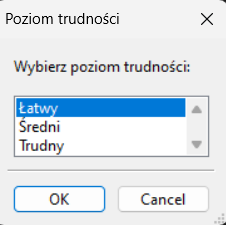
\includegraphics[width=\linewidth]{1.png}
	\caption{Wybór poziomu trudności}
	\label{rys:1}
	Jak widać na rysunku \ref{rys:1}, jest to wstępne okienko pojawiające się przed rozpoczęciem gry, aby dostosować poziom trudności, tym samym wybór bazy pytań. Gracz ma możliwość wyboru między różnymi poziomami trudności, co wpływa na zestaw pytań, z którymi będzie musiał się zmierzyć podczas gry. Opcje te pozwalają na dostosowanie gry do umiejętności i preferencji gracza, co zwiększa jej atrakcyjność i dostosowanie do indywidualnych potrzeb.
\end{figure}

\begin{figure}[!h]
	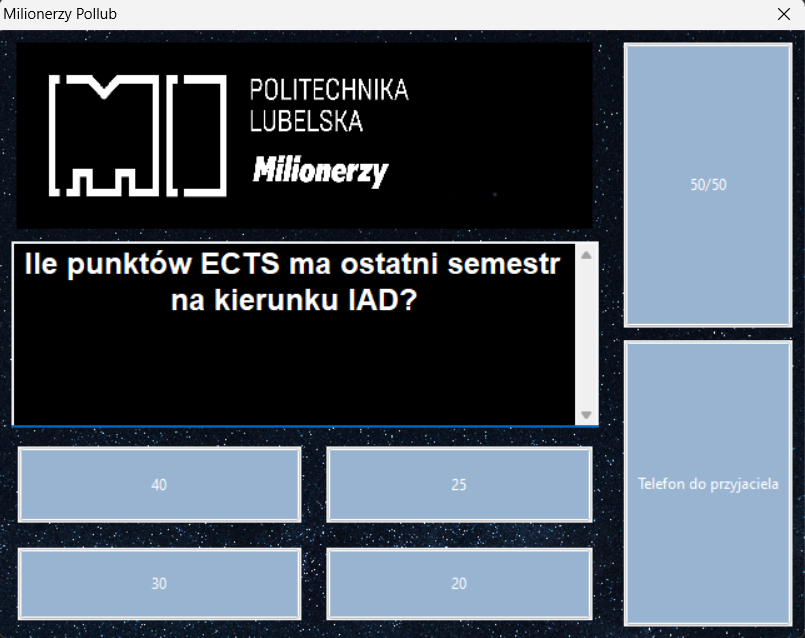
\includegraphics[width=\linewidth]{2.png}
	\caption{Interfejs startowy}
	\label{rys:2}
	Rysunek \ref{rys:2} przedstawia okno po uruchomieniu aplikacji w momencie startowym po wybraniu poziomu trudności. W tym wypadku został wybrany poziom trudności "łatwy", co powoduje, że widzimy skutek działania funkcji rysowania tła i losowania pytań.
\end{figure}

\begin{figure}[!h]
	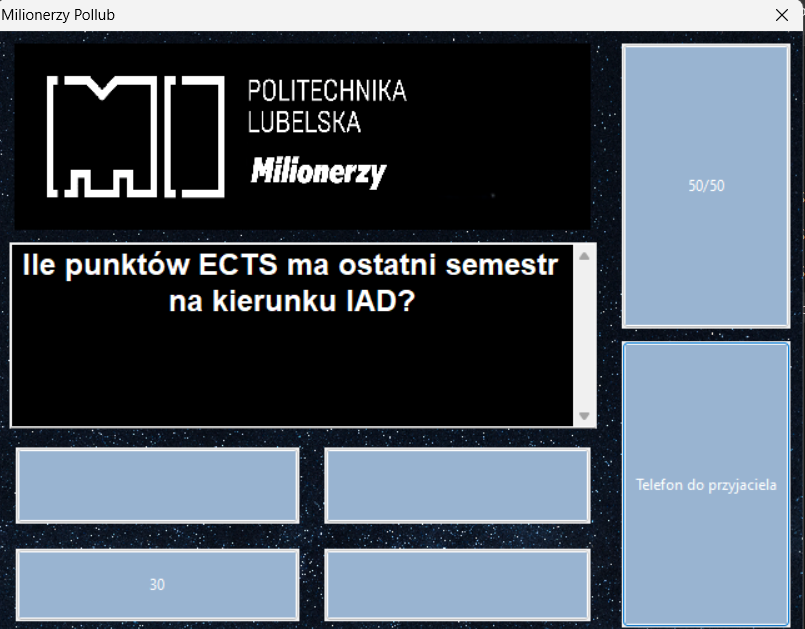
\includegraphics[width=\linewidth]{3.png}
	\caption{Koło ratunkowe telefon do przyjaciela}
	\label{rys:3}
	Na rysunku \ref{rys:3} pokazano sytuację, w której gracz używa koła ratunkowego "telefon do przyjaciela" w celu uzyskania pomocy przy odpowiedzi na pytanie. Jest to jedno z dostępnych kół ratunkowych, które gracz może wykorzystać w trudnych momentach gry. Wybór tego koła ratunkowego pozwala "skontaktować się z wirtualnym przyjacielem", który raz w całej grze może nam wskazać poprawną odpowiedź.
\end{figure}

\begin{figure}[!h]
	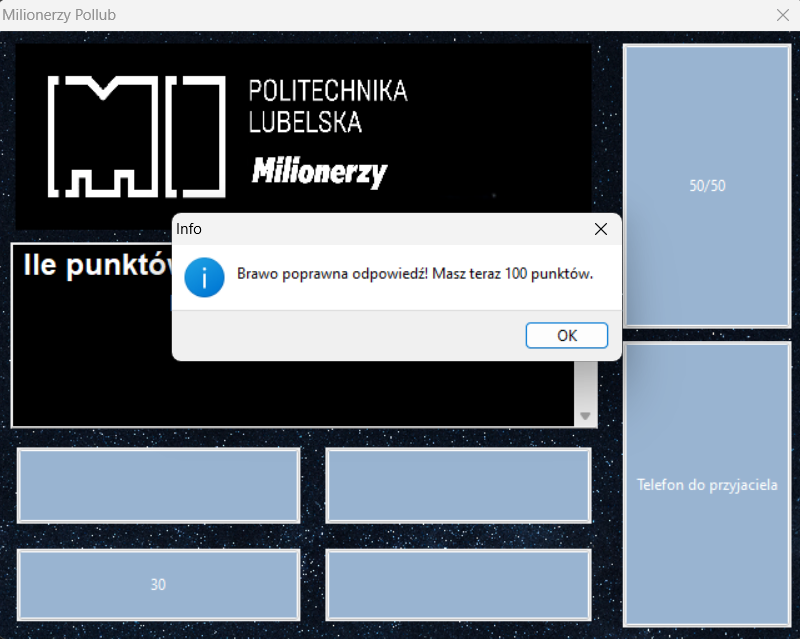
\includegraphics[width=\linewidth]{4.png}
	\caption{Wybranie poprawnej odpowiedzi}
	\label{rys:4}
	Rysunek \ref{rys:4} przedstawia moment, w którym gracz wybiera poprawną odpowiedź na zadane pytanie. Interfejs wyraźnie wskazuje, która odpowiedź została wybrana, a także informuje gracza o jej poprawności. Poprawne odpowiedzi są nagradzane i gracz zyskuje 100 pkt, co motywuje gracza do dalszej rozgrywki i zwiększa jego zaangażowanie w grę.
\end{figure}

\begin{figure}[!h]
	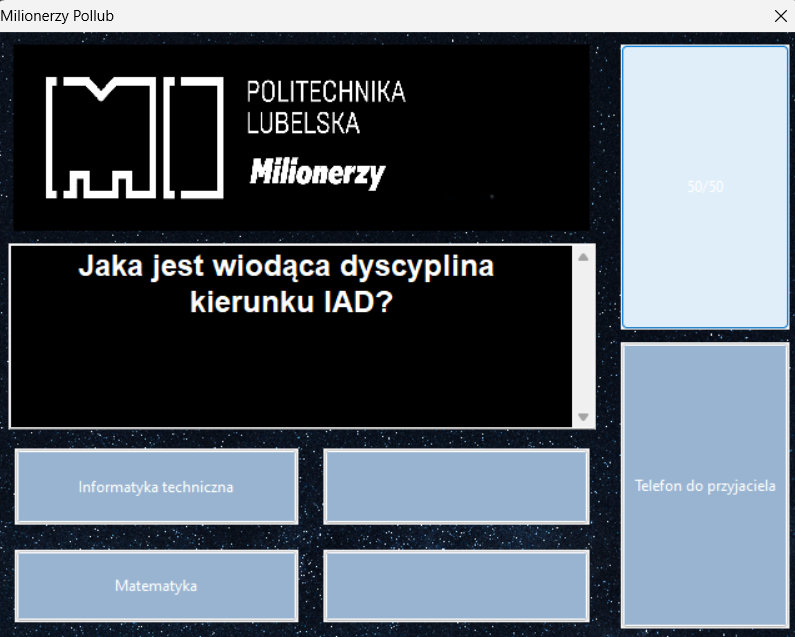
\includegraphics[width=\linewidth]{5.png}
	\caption{Koło ratunkowe 50/50}
	\label{rys:5}
	Na rysunku \ref{rys:5} widać użycie koła ratunkowego 50/50, które usuwa dwie błędne odpowiedzi, pozostawiając jedną poprawną i jedną niepoprawną odpowiedź. Jest to koło które znacząco zwiększa szanse gracza na udzielenie poprawnej odpowiedzi, zwłaszcza w trudniejszych pytaniach, gdzie pewność odpowiedzi jest niska. Te koło również możemy użyć tylko raz w ciągu całej gry.
\end{figure}

\begin{figure}[!h]
	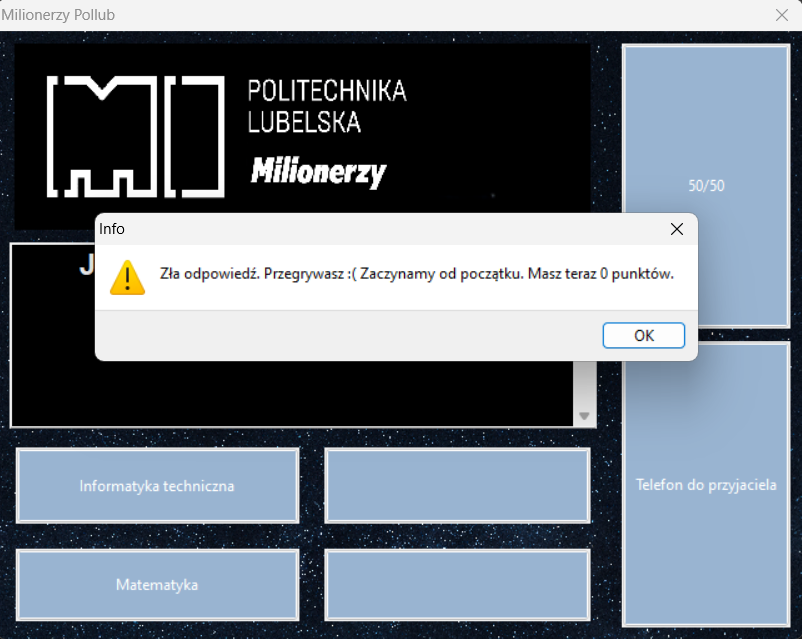
\includegraphics[width=\linewidth]{6.png}
	\caption{Komunikat o złej odpowiedzi}
	\label{rys:6}
	Rysunek \ref{rys:6} przedstawia komunikat, który pojawia się, gdy gracz udzieli niepoprawnej odpowiedzi na pytanie. Interfejs informuje gracza o błędnej odpowiedzi i przekazuje odpowiednie informacje zwrotne, o resetwaniu liczny punktów do 0 i ropzpoczęcie gry od początku na tym samym poziomie gry. Komunikat ten jest kluczowym elementem gry, który wpływa na doświadczenie użytkownika i jego zaangażowanie.
\end{figure}

\begin{figure}[!h]
	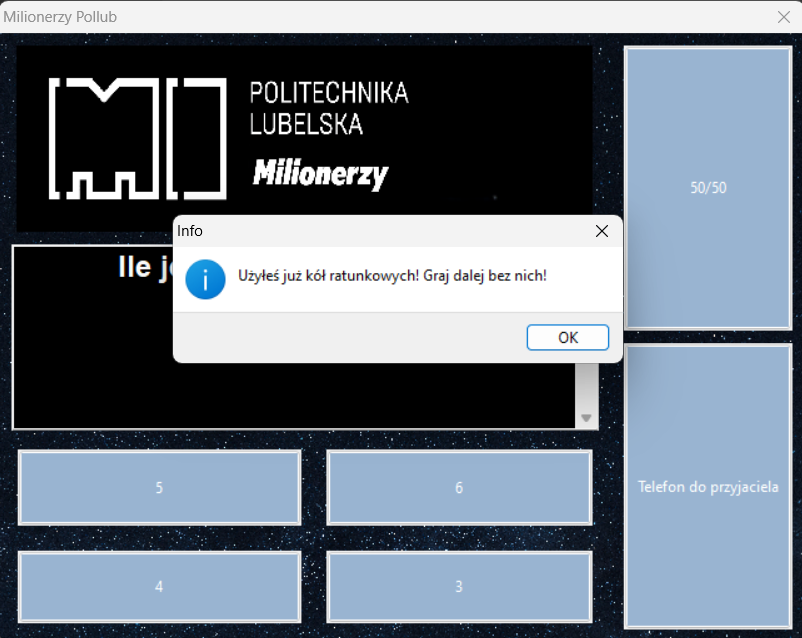
\includegraphics[width=\linewidth]{8.png}
	\caption{Komunikat o użyciu kół ratunkowych}
	\label{rys:7}
	Rysunek \ref{rys:7} pokazuje komunikat, który informuje gracza o użyciu wszystkich dostępnych kół ratunkowych. Jest to ważna informacja, ponieważ gracz musi być świadomy, że nie może już skorzystać z dodatkowej pomocy i musi polegać wyłącznie na swojej wiedzy w dalszej części gry. Komunikat ten motywuje do ostrożniejszego podejmowania decyzji w kolejnych rundach.
\end{figure}

\begin{figure}[!h]
	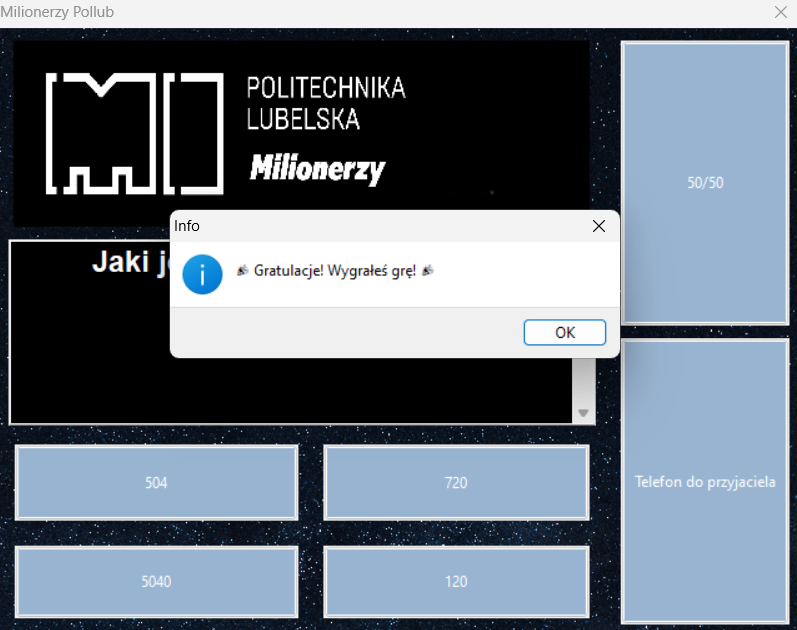
\includegraphics[width=\linewidth]{9.png}
	\caption{Komunikat o wygranej}
	\label{rys:8}
	Na rysunku \ref{rys:8} przedstawiono komunikat, który pojawia się, gdy gracz wygra grę tzn. uzyska 1000 pkt, udzielając poprawnej odpowiedzi na ostatnie pytanie. Komunikat ten informuje o zakończeniu gry i gratuluje graczowi osiągnięcia sukcesu. Jest to kluczowy moment gry, który nagradza gracza za jego wysiłek i wiedzę, zapewniając satysfakcję i pozytywne wrażenia z rozgrywki.
\end{figure}
\end{document}